\chapter{Tables and Figures}
In this chapter we will see some examples of tables and figures.

\section{Tables}
Let's see how to make a well designed table.

\begin{table}[tb]
\caption[A floating table]{A floating table.}
\label{tab:esempio}
\centering
\begin{tabular}{ccc}
\toprule
name & weight & food \\ 
\midrule
mouse	& 10 g	& cheese \\
cat	& 1 kg	& mice \\
dog	& 10 kg	& cats \\
t-rex	& 10 Mg	& dogs \\
\bottomrule 
\end{tabular}
\end{table}

The table~\ref{tab:esempio} is a floating table and was obtained with the following code:
\begin{lstlisting}
\begin{table}[tb]
\caption[A floating table]{A floating table.}
\label{tab:example}
\centering
\begin{tabular}{ccc}
\toprule
	name 	& weight & food	  \\ 
\midrule
	mouse	& 10  g	 & cheese \\
	cat		&  1 kg	 & mice	  \\
	dog		& 10 kg	 & cats   \\
	t-rex	& 10 Mg	 & dogs	  \\
\bottomrule 
\end{tabular}
\end{table}
\end{lstlisting}

\lipsum[1-2]


\section{Figures}
Let's see now how to put one or several images in your text.


\begin{figure}[tb] 
\centering 
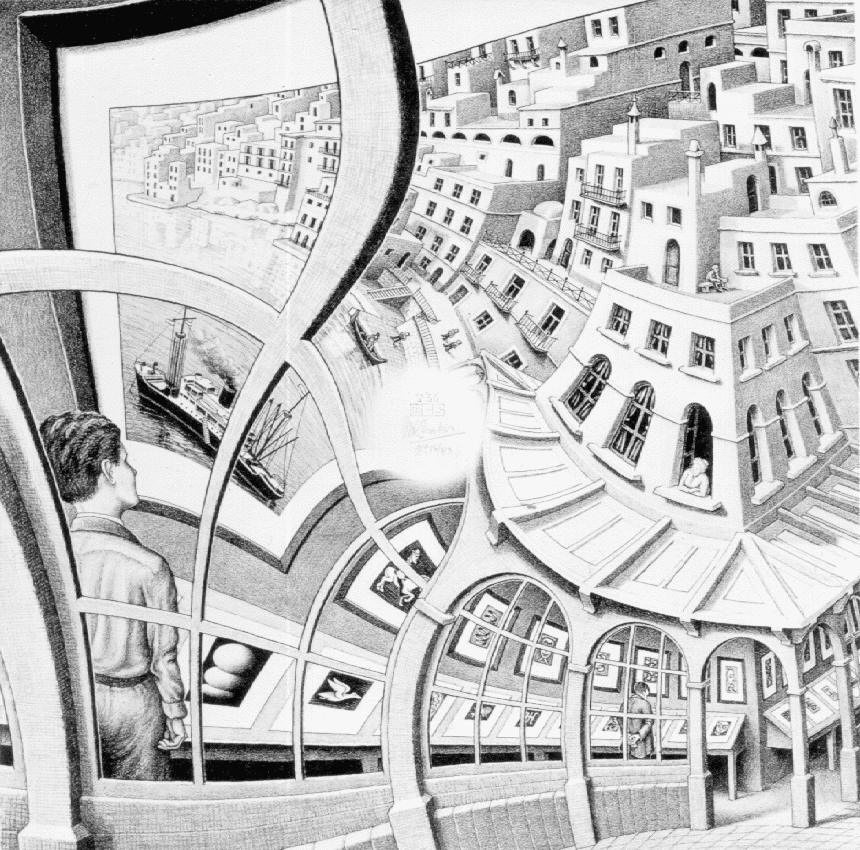
\includegraphics[width=0.5\columnwidth]{galleria_stampe} 
\caption[A floating figure]{A floating figure (the lithograph \emph{Galleria di stampe}, of M.~Escher, got from \url{http://www.mcescher.com/}).}
\label{fig:galleria} 
\end{figure}

\begin{figure}[tb] 
\centering 
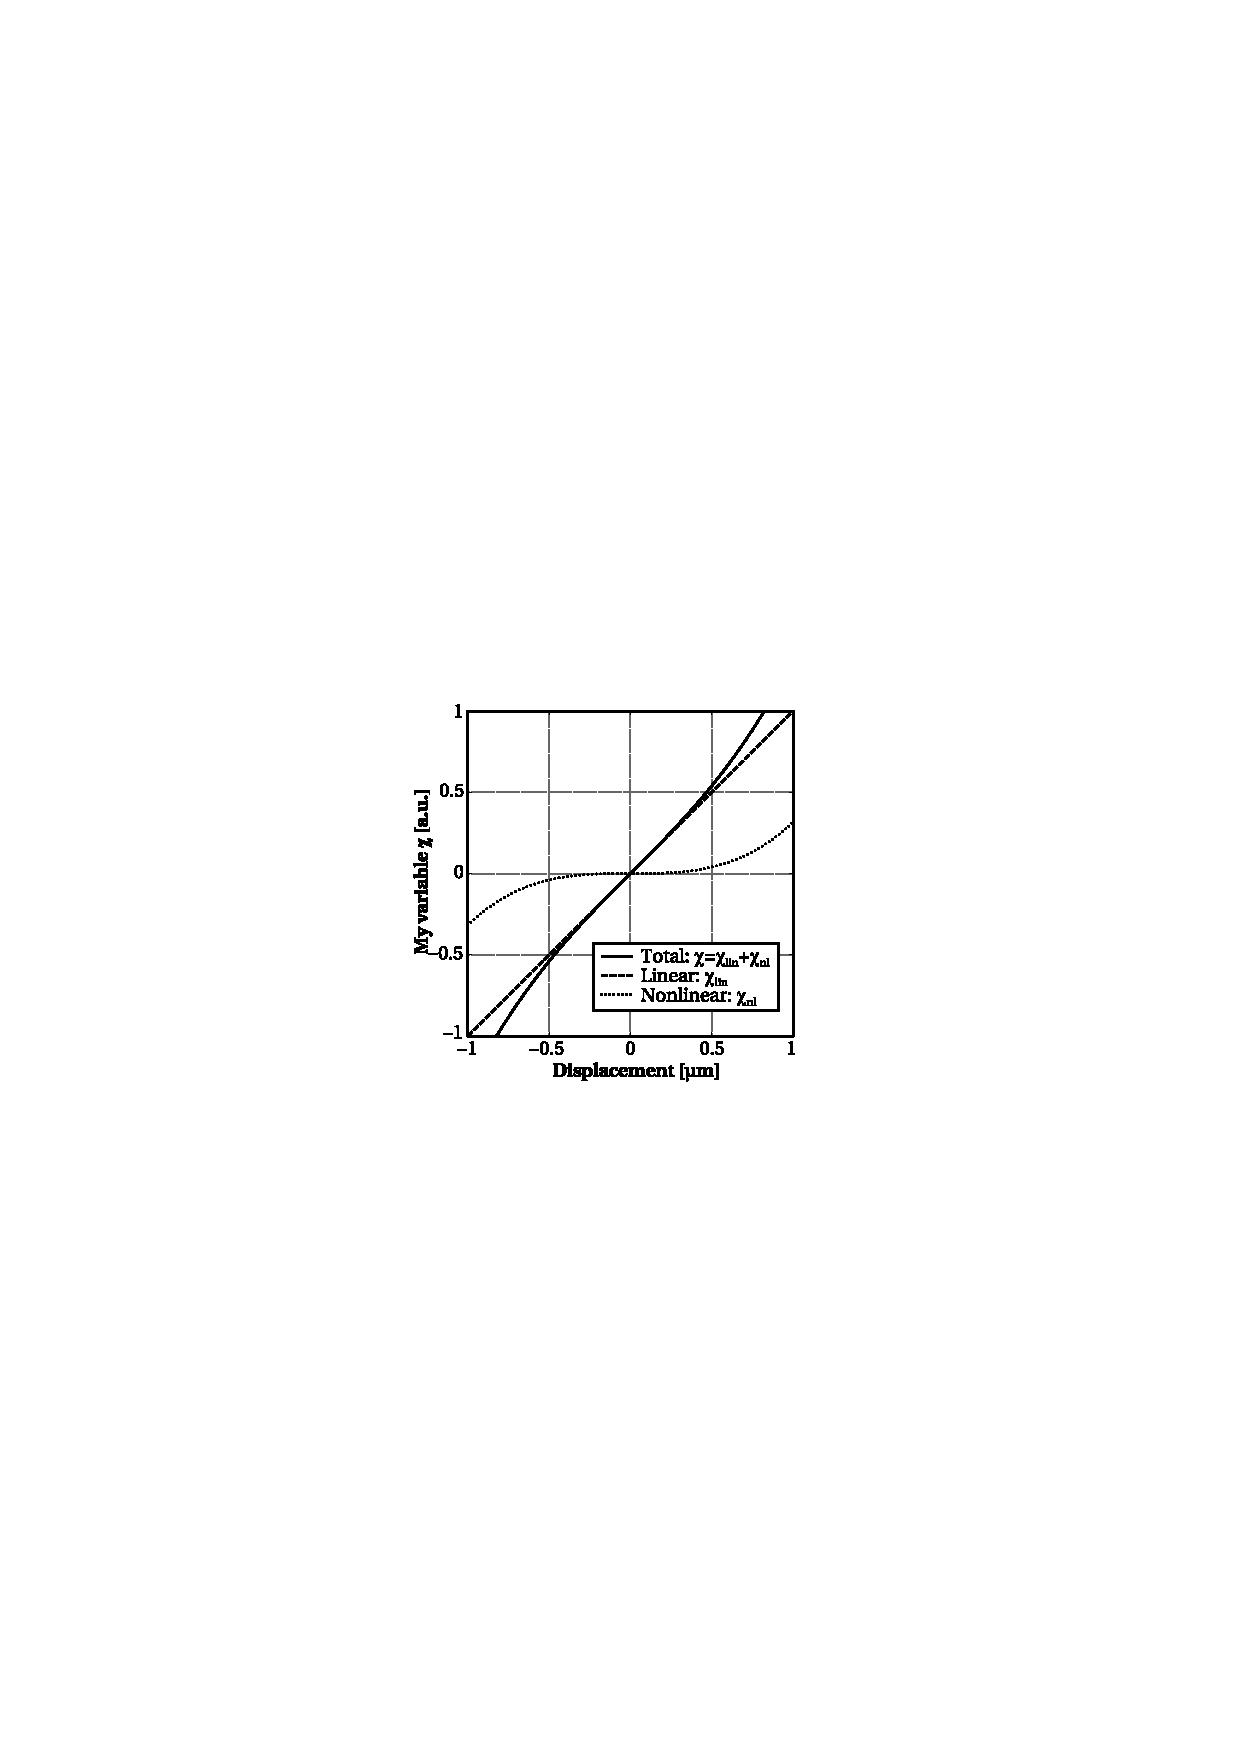
\includegraphics{some_vector_graphics.pdf} 
\caption[A floating figure]{A floating figure with text typeset in "Utopia Latex", a font provided in the template-folder for typesetting figures with greek characters. The text has been "outlined" for best compatibility with the repro during the printing.}
\label{fig:vector_graphics} 
\end{figure}


The figure~\ref{fig:galleria} is a floating figure and was obtained with the following code:
\begin{lstlisting}
\begin{figure}[tb] 
\centering 
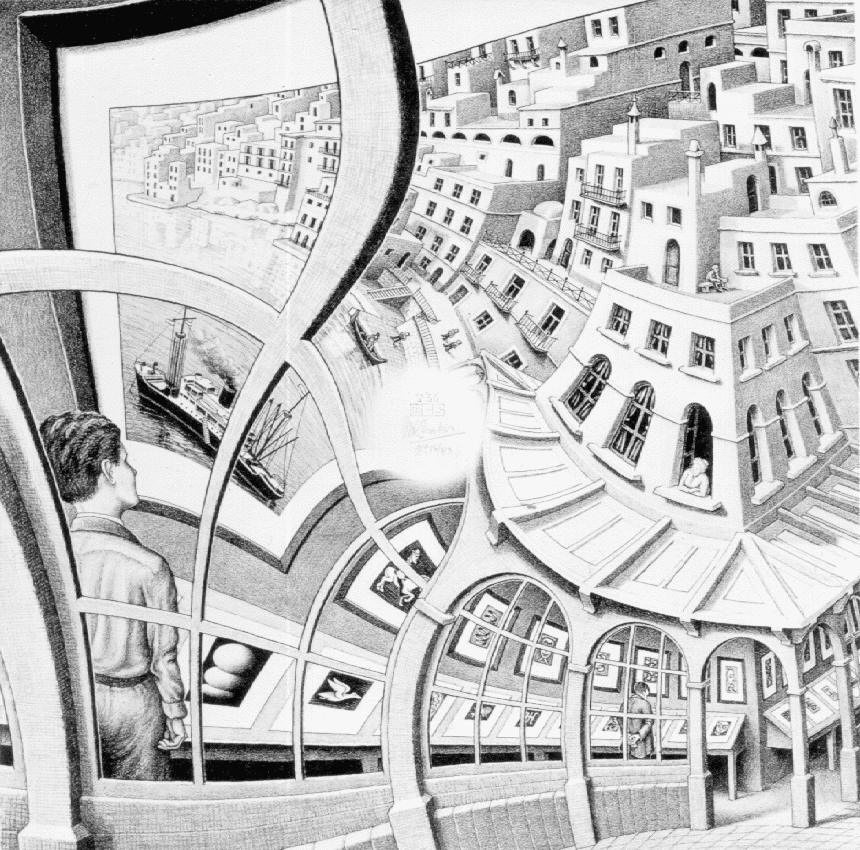
\includegraphics[width=0.5\columnwidth]{galleria_stampe} 
\caption[A floating figure]{A floating figure ... }
\label{fig:galleria} 
\end{figure}
\end{lstlisting}


\lipsum[1-2]

\begin{figure}[tb]
\centering

\subfloat[Asia personas duo.]
{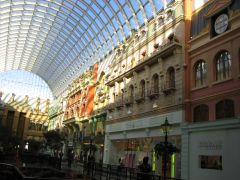
\includegraphics[width=.45\columnwidth]{lorem}} \quad
\subfloat[Pan ma signo.]
{\label{fig:ipsum}%

\includegraphics[width=.45\columnwidth]{ipsum}} \\
\subfloat[Methodicamente o uno.]
{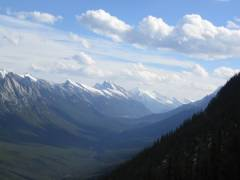
\includegraphics[width=.45\columnwidth]{dolor}} \quad
\subfloat[Titulo debitas.]
{
\includegraphics[width=.45\columnwidth]{sit}}
\caption[Tu duo titulo debitas latente]{Tu duo titulo debitas
latente.}
\label{fig:esempio}
\end{figure}

The figure~\ref{fig:esempio} is a floating figure and was obtained with the following code:
\begin{lstlisting}
\begin{figure}[tb]
\centering
\subfloat[Asia personas duo.]
{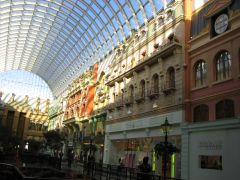
\includegraphics[width=.45\columnwidth]{lorem}} \quad
\subfloat[Pan ma signo.]
{\label{fig:ipsum}%

\includegraphics[width=.45\columnwidth]{ipsum}} \\
\subfloat[Methodicamente o uno.]
{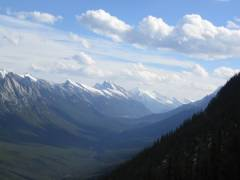
\includegraphics[width=.45\columnwidth]{dolor}} \quad
\subfloat[Titulo debitas.]
{
\includegraphics[width=.45\columnwidth]{sit}}
\caption[Tu duo titulo debitas latente]{Tu duo titulo debitas latente.}
\label{fig:esempio}
\end{figure}
\end{lstlisting}


\lipsum[3-8]
